\section{Prezentacja aplikacji}

\begin{frame}{\insertsection}
	\only<1>{
		\begin{block}{Formularz logowania}
			Aplikacja webowa wymaga autoryzacji.
		\end{block}
	}
	\only<2>{
	\begin{block}<2>{Tłumaczenie}
		Możliwość presonalizacji języka.
	\end{block}
	}
	\begin{columns}
		\column{0.5\textwidth} 
		\begin{figure}
			\centering
			\includegraphics[width=1\linewidth]{../images/login.png}
		\end{figure}
		\column{0.5\textwidth} 
		\begin{figure}
			\centering
			\includegraphics[width=1\linewidth]{../images/loginang.png}
		\end{figure}
	\end{columns}
\end{frame}

\begin{frame}{\insertsection}
	\begin{columns}
		\column{0.5\textwidth} 
		\begin{block}{Formularz rejestracji}
			Istnieje możliwość utworzenia konta.
		\end{block}
		\column{0.5\textwidth} 
		\begin{figure}
			\centering
			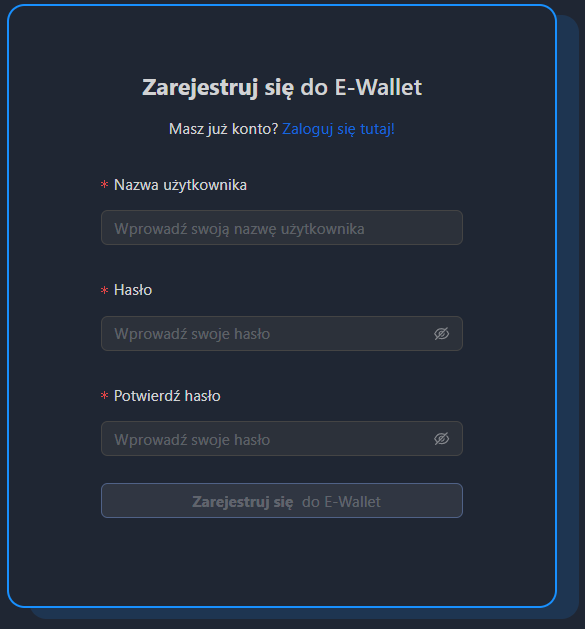
\includegraphics[width=1\linewidth]{../images/Rejestracja}
			\label{fig:rejestracja}
		\end{figure}
	\end{columns}
\end{frame}

\begin{frame}{\insertsection}
	\begin{block}{Strona główna}
		Umożliwia sprawdzanie informacji o kontach	
	\end{block}
	\begin{figure}
		\centering
		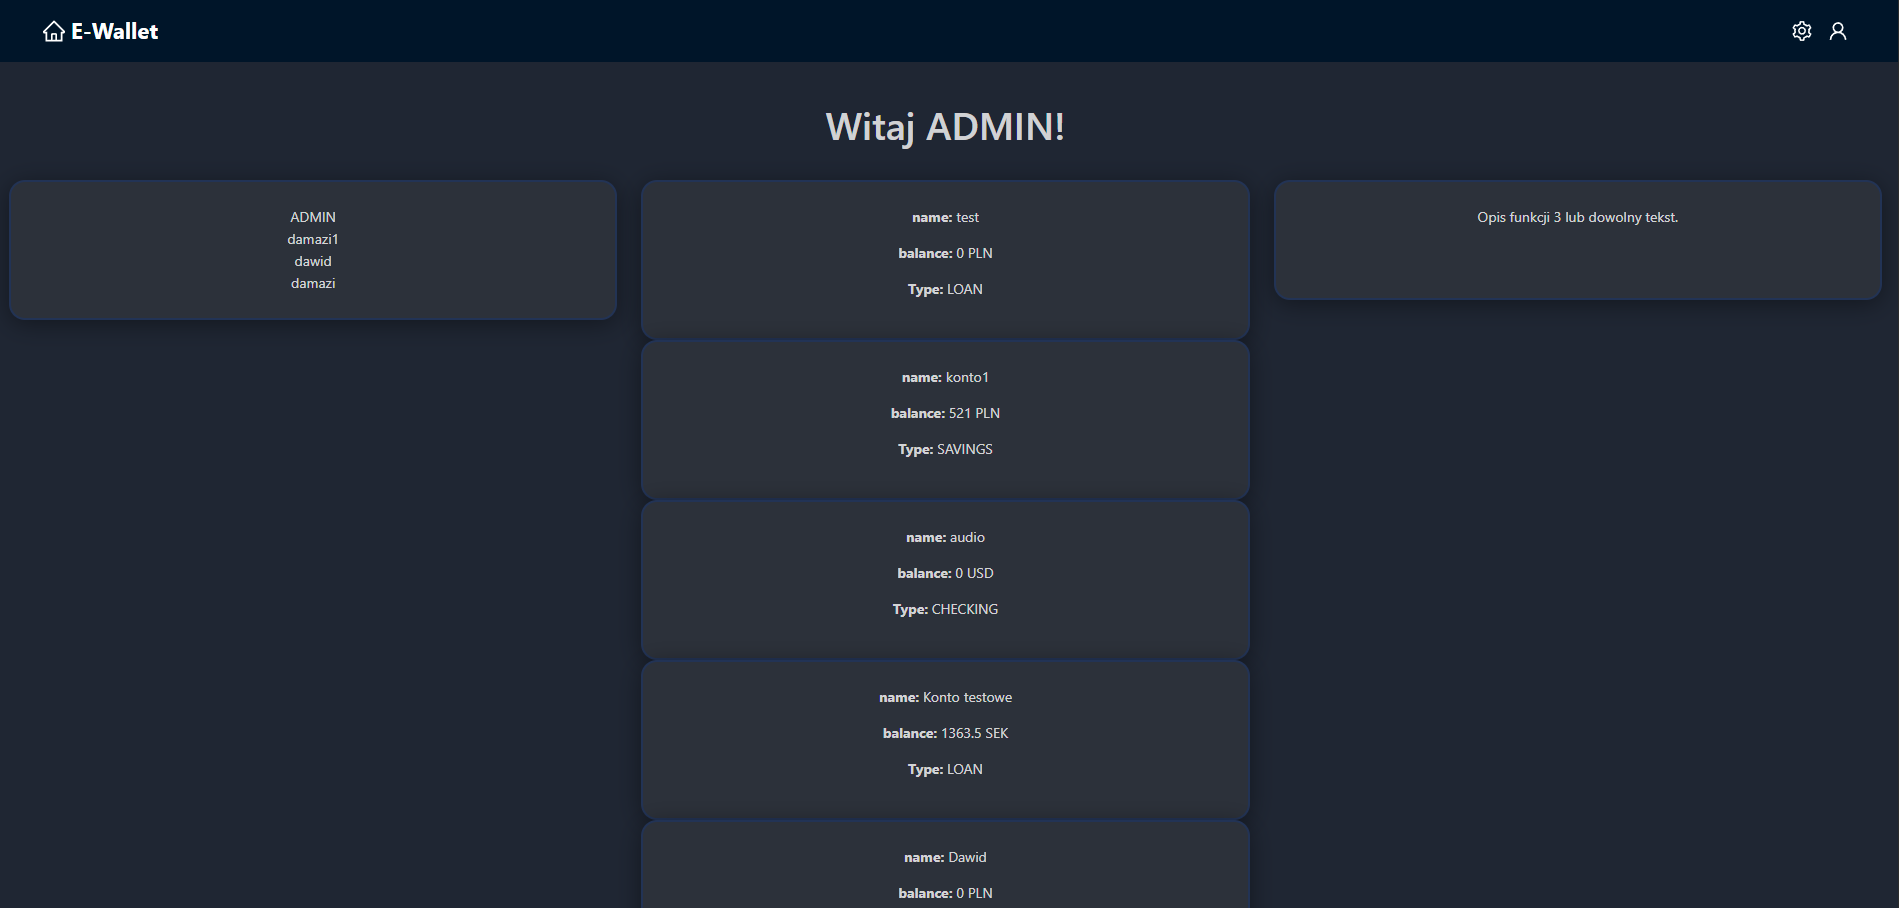
\includegraphics[width=0.9\linewidth]{../images/MotywCiemny}
	\end{figure}
\end{frame}

\begin{frame}{\insertsection}
	\begin{block}{Wybór motywu}
		Personalizacja barw aplikacji.
	\end{block}
		\begin{figure}
		\centering
		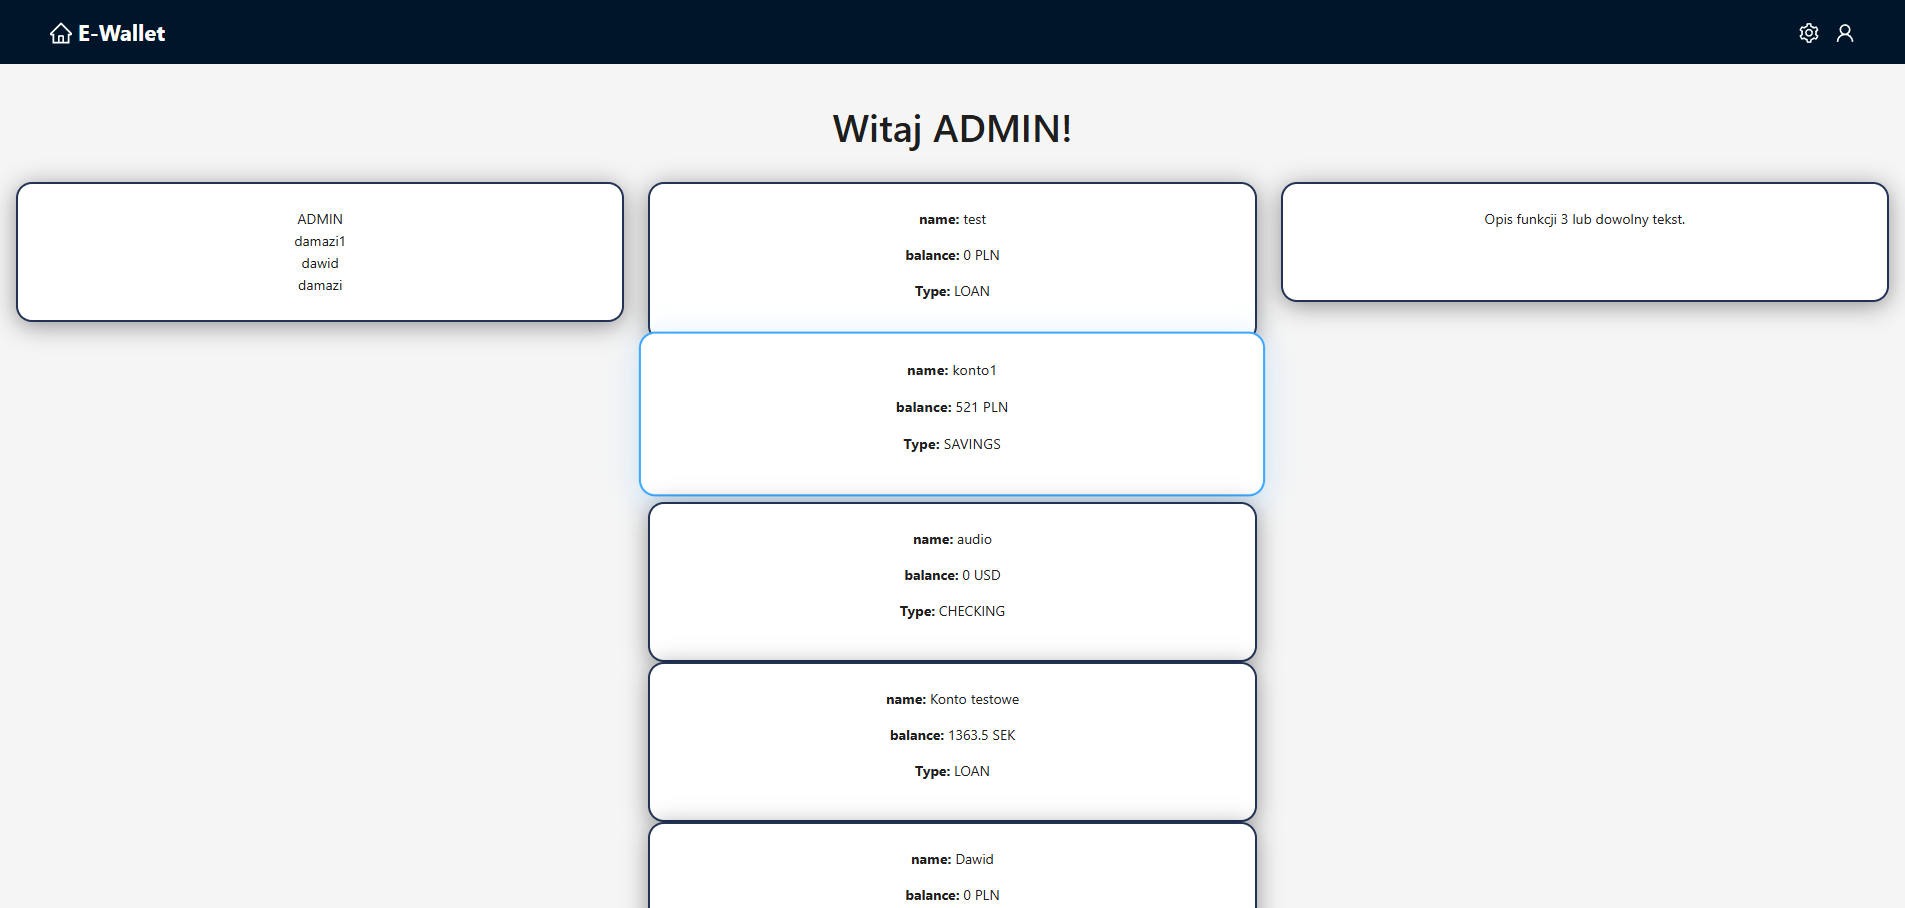
\includegraphics[width=0.9\linewidth]{../images/MotywJasny}
	\end{figure}
\end{frame}

\begin{frame}{\insertsection}
	\begin{columns}
		\column{0.45\textwidth} 
		\begin{block}{Pasek nawigacyjny}
			Udostępnia możliwość powrotu do strony głównej, dostęp do ustawień oraz wyświetlania danych użytkownika.
		\end{block}
		\begin{figure}
			\centering
			
\includegraphics[width=0.7\linewidth]{../images/Navbar}
			\caption{Navbar}
			\label{fig:navbar}
		\end{figure}
		\column{0.45\textwidth} 
		\begin{block}{Ustawienia}
			Pozwala na wybór języka i motywu.
		\end{block}
		\begin{figure}
			\centering
			
\includegraphics[width=0.7\linewidth]{../images/Ustawienia}
			\caption{Ustawienia}
			\label{fig:ustawienia}
		\end{figure}	
	\end{columns}
\end{frame}

\begin{frame}{\insertsection}
	\begin{block}{Detale konta}
		Udostępnia informacje o użytkowniku
	\end{block}
	\begin{figure}
		\centering
		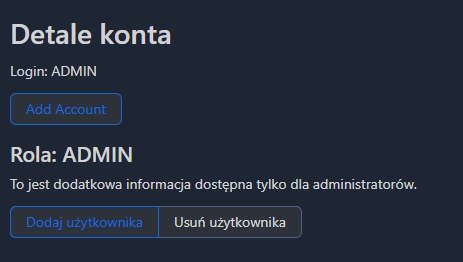
\includegraphics[width=0.7\linewidth]{../images/DetaleKonta}
		\label{fig:detalekonta}
	\end{figure}
\end{frame}

\begin{frame}{\insertsection}
\begin{columns}[t] % kolumny wyrównane do góry
	\column{0.33\textwidth}
	% minipage o stałej wysokości (tu 4.5cm) - w środku obraz wycentrowany, podpis poniżej (na stałej pozycji)
	\begin{minipage}[t][4.5cm][c]{\linewidth}
		\centering
		\adjustbox{valign=c}{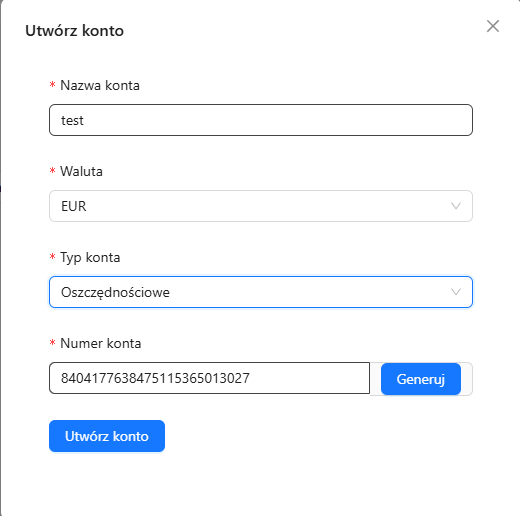
\includegraphics[width=\linewidth,keepaspectratio]{../images/AccountForm}}
	\end{minipage}
	\vspace{0.6ex}
	\captionof{figure}{Dodawanie konta}
	
	\column{0.33\textwidth}
	\begin{minipage}[t][4.5cm][c]{\linewidth}
		\centering
		\adjustbox{valign=c}{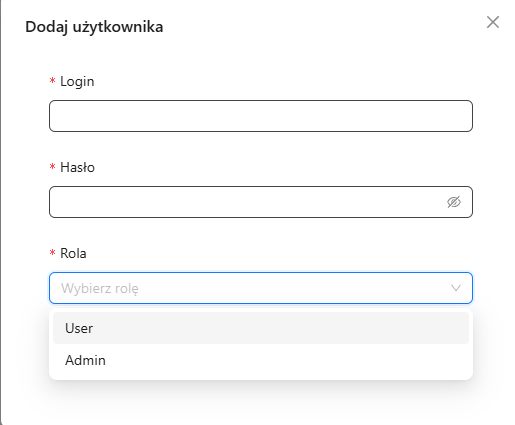
\includegraphics[width=\linewidth,keepaspectratio]{../images/DodawanieUzytkownika}}
	\end{minipage}
	\vspace{0.6ex}
	\captionof{figure}{Dodawanie użytkownika}
	
	\column{0.33\textwidth}
	\begin{minipage}[t][4.5cm][c]{\linewidth}
		\centering
		\adjustbox{valign=c}{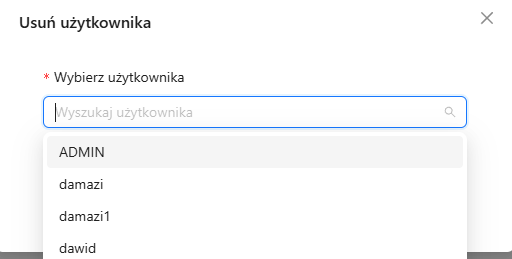
\includegraphics[width=\linewidth,keepaspectratio]{../images/UsuwanieUzytkownika}}
	\end{minipage}
	\vspace{0.6ex}
	\captionof{figure}{Usuwanie użytkownika}
\end{columns}
\end{frame}

\begin{frame}{\insertsection}
	\begin{block}{Detale portfela}
		Wyświetlanie danych o wpłatach i wypłatach.
	\end{block}
	\begin{columns}
		\column{0.45\textwidth}
			\begin{figure}
			\centering
			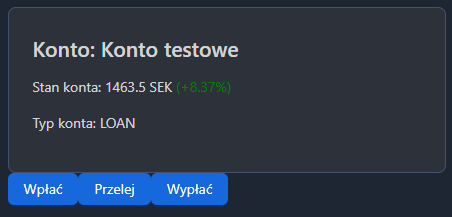
\includegraphics[width=1\linewidth]{../images/DanePortfela}
			\label{fig:daneportfela}
		\end{figure}
		\column{0.45\textwidth}
		\begin{figure}
			\centering
			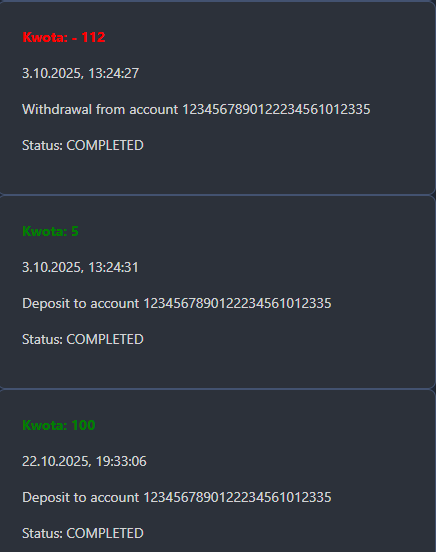
\includegraphics[width=0.9\linewidth]{../images/TransakcjeHistoria}
			\label{fig:transakcjehistoria}
		\end{figure}
		
	\end{columns}

\end{frame}

\begin{frame}{\insertsection}
\begin{figure}
	\centering
	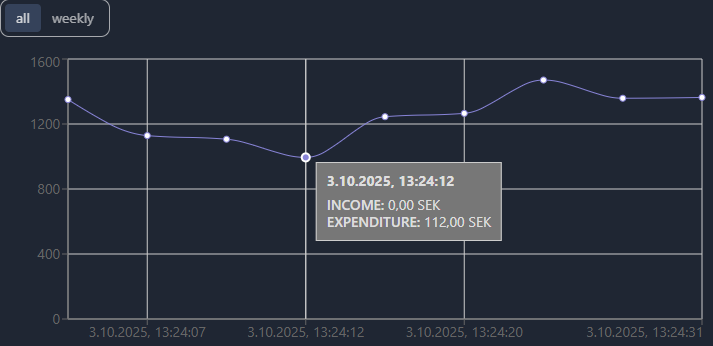
\includegraphics[width=1\linewidth]{../images/TransakcjeAll}
	\caption{Wszystkie wpłaty i wypłaty}
	\label{fig:transakcjeall}
\end{figure}
\end{frame}

\begin{frame}{\insertsection}
\begin{figure}
	\centering
	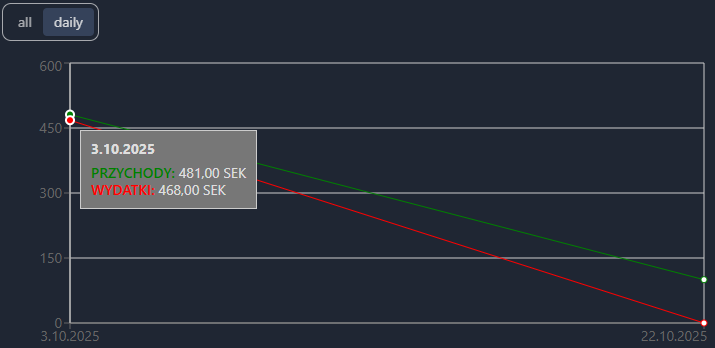
\includegraphics[width=1\linewidth]{../images/TransakcjeDaily}
	\caption{Wpłaty i wypłaty za poszczególne dni}
	\label{fig:transakcjedaily}
\end{figure}
\end{frame}
